\section{Likformig rörelse}
En likformig rörelse är en rörelse som genomförs med konstant hastighet i jämvikt. Den kan egentligen sammanfattas med den så kallade ''SVT-trianglen'':
\begin{figure*}[h]
    \centering
    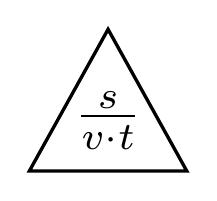
\begin{tikzpicture}[scale=2, every node/.style={scale=2}]
        \draw[very thick] (-0.5,-0.5) -- (0,-0.5) node[anchor=south, align=center] {\(\frac{s}{v \cdot t}\)} -- (0.5,-0.5) -- (0,0.4) -- cycle;
    \end{tikzpicture}
\end{figure*}

Denna kan användas genom att täcka för den sökta enheten med ett finger. och sedan kommer formel för den övertäcka enheten bli kvar. Sammanfattat gäller följande formler:
\begin{align*}
    s &= v \cdot t \\
    v &= \frac{s}{t} \\
    t &= \frac{s}{v} \\
\end{align*}

\section{Likformigt accelererande rörelse}
Om hastigheten inte längre är konstant är den enklaste nästa steg att accelerationen $a$ är konstant. då gäller följande formler:
\begin{align*}
    s &= \frac{at^2}{2} + v_0t + s_0 \\
    v &= at + v_0 
\end{align*}

\section{Allmän rörelse}
All rörelse kan beskrivas med hjälp av de ovanstående formlerna men man måste blanda in lite integral- och differentialkalkyl. För att uppnå denna fullständinga definition vill vi först tänka på rörelsens storheter som funktioner av tiden:
\begin{equation*}
    s(t) \text{ för sträcka, } v(t) \text{ för hastighet och } a(t) \text{ för accelration.}
\end{equation*}
Med detta kan vi sedan beräkna deras relation i alla möjliga fall. Här antar jag att du är bekant med tanken bakom integraler och derivator så här är snabbversionen av alla generella formler givet att $a(t)$ är linjärt:
\begin{align*}
    s(t) &= \frac{kt^3}{6} + \frac{a_0t^2}{2} + v_0t + s_0 \\
    v(t) &= \frac{kt^2}{2} + a_0t + v_0 \\
    a(t) &= kt + a_0
\end{align*}
eftersom
\begin{align*}
    v(t) &= s'(t) \\
    a(t) &= v'(t) = s''(t) \\
    s(t) &= \hyperref[def:indefint]{\int} {v(t)}\, dt = \iint{a(t)}\, dt\, dt
\end{align*}
(För fullständig härledning och teckenförklaring se bilaga \ref{derive:allmänrörelse}) Utifrån detta kan vi nu beräkna all rörelse bara vi vet formeln för en av storheterna. Om det inte finns en formel ska den hittas experimentellt eller så går det inte. Man kan sätta in valfri funktion för $a(t)$ och om man integrerar korrekt får man ändå rätt svar så detta är verkligen en allmän metod.

\section{Rörelsemängd}
Ett föremåls rörelsemängd är dess hastighet multiplicerat med dess massa och beteckans $p$. Formeln är: \[ p = mv\, \left[\mathrm{\frac{kg \cdot m}{s}  = kgm/s = N \cdot s}\right]\] Likt hastigheten är detta en vektor och har därför en riktning. Rörelsemängden skiljer sig från rörelseenergin $E_k$ eftersom $p \hyperref[def:propto]{\propto} v$ medan $E_k \propto v^2$.
\subsection{Stötar}
När två föremål krockar, dvs. stöter in i varandra så sker det ett utbyte av rörelsemängd. Rörelsemängden bevaras alltid enligt \emph{lagen om rörelsemängdens bevarande} (se bilaga \ref{derive:conserverationmomentum}). Rörelseenergin i systemet före och efter stöt är dock inte alltid konstant. (se \vref{tab:stötar}).
\begin{table*}[h]
    \centering
    \begin{tabular}{|>{\centering\arraybackslash}m{0.4\textwidth}|>{\centering\arraybackslash}m{0.4\textwidth}|}
        \hline
        Elastisk stöt          & Oelastisk stöt \\ \hline


        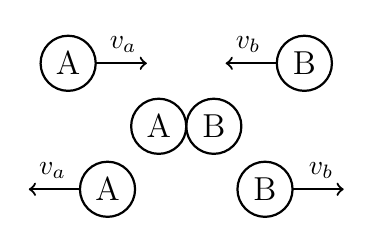
\begin{tikzpicture}[every path/.style={thick}]
            \vspace{8pt}
            \draw (-1.5,0) circle[radius=0.35cm] node {\large{A}};
            \draw[->] (-1.15, 0) -- ++(0.65,0) node[anchor=south east] {$v_a$};
            \draw (1.5,0) circle[radius=0.35cm] node {\large{B}};
            \draw[->] (1.15, 0) -- ++(-0.65,0) node[anchor=south west] {$v_b$};
            
            \draw (-0.35,-0.8) circle[radius=0.35cm] node {\large{A}};
            \draw (0.35,-0.8) circle[radius=0.35cm] node {\large{B}};
            
            \draw (-1,-1.6) circle[radius=0.35cm] node {\large{A}};
            \draw (1,-1.6) circle[radius=0.35cm] node {\large{B}};
            \draw[->] (-1.35,-1.6) -- ++(-0.65,0) node[anchor=south west] {$v_a$};
            \draw[->] (1.35,-1.6) -- ++(0.65,0) node[anchor=south east] {$v_b$};
            \vspace{8pt}
        \end{tikzpicture} & 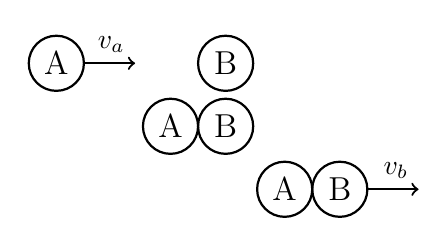
\begin{tikzpicture}[every path/.style={thick}]
            \vspace{8pt}
            \draw (-1.8,0) circle[radius=0.35cm] node {\large{A}};
            \draw[->] (0.35-1.8,0) -- ++(0.65,0) node[anchor=south east] {$v_a$};
            \draw (0.35,0) circle[radius=0.35cm] node {\large{B}};
            
            \draw (-0.35,-0.8) circle[radius=0.35cm] node {\large{A}};
            \draw (0.35,-0.8) circle[radius=0.35cm] node {\large{B}};
            
            \draw (1.8-0.35*2,-1.6) circle[radius=0.35cm] node {\large{A}};
            \draw (1.8,-1.6) circle[radius=0.35cm] node {\large{B}};
            \draw[->] (1.8+0.35,-1.6) -- ++(0.65,0) node[anchor=south east] {$v_b$};
            \vspace{8pt}
        \end{tikzpicture} \\ \hline


        Rörelseenergin bevaras & Rörelseenergin bevaras inte \\ \hline
    \end{tabular}
    \caption{Stötar}
    \label{tab:stötar}
\end{table*}
\subsubsection{Elastiskta stötar}
Vid s.k. \emph{elastiska stötar} bevaras rörelseenergin i systemet. Detta beror på att en elastisk stöt är definierad som en stöt där ingen energi gå förlorat till ex. värme. Sambandet som vi får för elastiska stötar enligt lagen om rörelsemängdens bevarande är då:
\begin{equation*}
    m_au_a + m_bu_b = m_av_a + m_bv_b
\end{equation*} 
där $u_a$ och $u_b$ är hastigheterna innan och $v_a$ och $v_b$ är hastigheterna efter. 

Detta är såklart enbart möjligt teoretisk så rörelseenergin bevaras bara helt i teorin. Det enda stället en fullständigt elastisk stöt kan ske är när föremålen inte nuddar varandra i ett vakum alltså exempelvis elementarpartiklar i rymden. I verkligheten är det närmaste vi kommer någonting liknande är billiardklot. Många krockar i både boken och på prov kan dock ses som fullständigt elastiska när uppgiften kräver det.
\subsubsection{Oelastiska stötar}
En \emph{oelastisk stöt} definieras som en stöt där en del av rörelseenergin omvandlas till andra energiformer som ex. värme genom ex. friktion. Detta innebär att den totala energin i systemet bevaras enligt energiprincipen men rörelseenergin efter stöten är inte samma som från början. Föremålen kommmer även att bli ''förenade'', dvs. ses som ett föremål med en sammanlagd massa. Givet lagen om rörelsemängdens bevarande gäller sambandet:
\begin{equation*}
    m_au_a + m_bu_b = (m_a + m_b)v
\end{equation*}
med $u_a$ och $u_b$ som hastigheterna innan stöten och $v$ som hastigheten efter stöten. Rörelsemängden bevaras alltså oavsett vad, men rörelseenergin är inte alltid densamma före och efter.